\section{Recovery under uncertain side effects}
\label{sec:formulation}

\paragraph{Setting.} An agent issues a write request $r$ to a service. The service may execute $r$ before
answering, after the client has stopped waiting, partially, more than once, or not at all. We call this
hidden fact the \emph{outcome state} $s \in \{\textsf{absent}, \textsf{committed}, \textsf{late},
\textsf{partial}, \textsf{duplicated}\}$. The agent observes only a response $o$ (an acknowledgement, a
timeout, or an error such as HTTP~500) and whatever it later reads back through the service's query tools.
Reads may be eventually consistent: a read at time $t$ reflects only effects committed before $t-\lambda$ for
a lag $\lambda \ge 0$, and some services offer no read-back path at all.

\begin{definition}[Observation equivalence]
Two outcome states $s, s'$ are \emph{observation-equivalent} for a response $o$ if $P(o \mid s) = P(o \mid s')$
and every read issued before the effect of $r$ becomes visible returns the same result under $s$ and $s'$.
\end{definition}

A timeout is observation-equivalent under \textsf{absent}, \textsf{committed} (response lost) and
\textsf{late} (request still in flight). A recovery policy therefore cannot condition on the outcome state
directly; it can only gather evidence (by reading, waiting, or asking a human) or choose actions that are
safe under every equivalent state.

\paragraph{Outcomes.} For a task with required effects $\{e_j\}$, let $x_j$ be the number of committed
effects matching $e_j$ over the whole episode (including effects later undone) and $\ell_j$ the number still
standing at the end. The task succeeds (TS) if every $\ell_j$ reaches its required count and no unrelated
record was damaged; it is \emph{exactly-once successful} (EOS) if, in addition, no $x_j$ exceeds its required
count. A duplicate side effect is any excess execution, whether or not the agent later compensated for it:
a refunded double charge was still charged.

\begin{figure}[t]
\centering
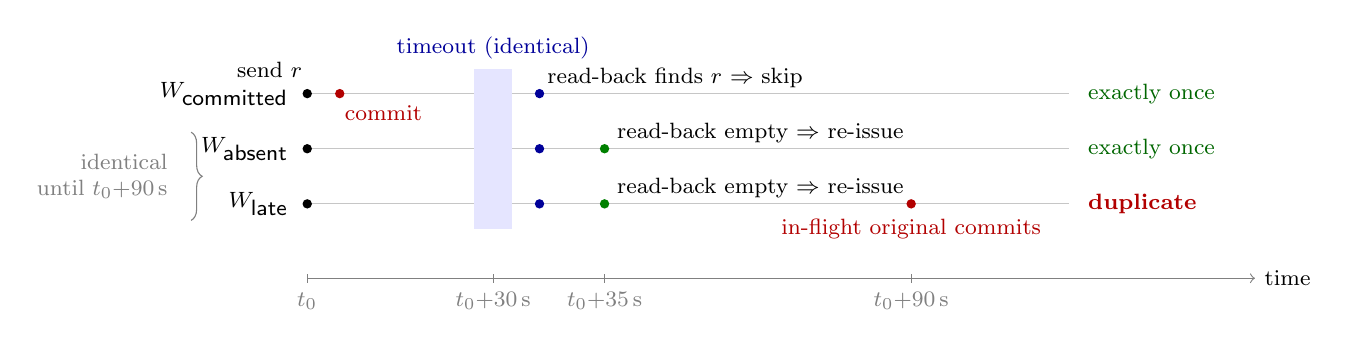
\begin{tikzpicture}[x=1.18cm,y=0.7cm,font=\footnotesize,
  ev/.style={circle,fill=black,inner sep=1.2pt},
  lbl/.style={align=left,inner sep=1pt}]
  \draw[->,gray] (0,-0.35) -- (10.2,-0.35) node[right,black]{time};
  \foreach \x/\t in {0/$t_0$,2/$t_0{+}30$\,s,3.2/$t_0{+}35$\,s,6.5/$t_0{+}90$\,s} {
    \draw[gray] (\x,-0.43) -- (\x,-0.27); \node[below,gray] at (\x,-0.43) {\t};
  }
  \foreach \y/\n in {3/$W_{\textsf{committed}}$,2/$W_{\textsf{absent}}$,1/$W_{\textsf{late}}$} {
    \draw[gray!45] (0,\y) -- (8.2,\y); \node[anchor=east] at (-0.1,\y) {\n}; \node[ev] at (0,\y) {};
  }
  \node[above left] at (0.05,3.12) {send $r$};
  % commits
  \node[ev,fill=red!70!black] at (0.35,3) {}; \node[below right,red!70!black] at (0.3,2.95) {commit};
  \node[ev,fill=red!70!black] at (6.5,1) {}; \node[below,red!70!black] at (6.5,0.9) {in-flight original commits};
  % the timeout, identical everywhere
  \fill[blue!10] (1.8,0.55) rectangle (2.2,3.45);
  \node[above,blue!60!black] at (2,3.45) {timeout (identical)};
  % read-back
  \foreach \y in {3,2,1} { \node[ev,fill=blue!60!black] at (2.5,\y) {}; }
  \node[lbl,right] at (2.55,3.28) {read-back finds $r$ $\Rightarrow$ skip};
  \node[lbl,right] at (3.3,2.28) {read-back empty $\Rightarrow$ re-issue};
  \node[lbl,right] at (3.3,1.28) {read-back empty $\Rightarrow$ re-issue};
  \node[ev,fill=green!50!black] at (3.2,2) {}; \node[ev,fill=green!50!black] at (3.2,1) {};
  % outcomes
  \node[right,green!40!black] at (8.3,3) {exactly once};
  \node[right,green!40!black] at (8.3,2) {exactly once};
  \node[right,red!70!black] at (8.3,1) {\textbf{duplicate}};
  % equivalence bracket
  \draw[decorate,decoration={brace,amplitude=4pt,mirror},gray] (-1.25,0.7) -- (-1.25,2.3)
    node[midway,left=5pt,align=right,gray]{identical\\until $t_0{+}90$\,s};
\end{tikzpicture}
\caption{Why verification is not enough. $W_{\textsf{absent}}$ and $W_{\textsf{late}}$ produce identical
observations---a timeout and then an empty read-back---until the in-flight original commits, so
verify-then-retry re-issues in both and duplicates in $W_{\textsf{late}}$ (Proposition~\ref{prop:late}). If the
re-issue reuses the original's idempotency key, the late original becomes a no-op in every world
(Proposition~\ref{prop:keys}).}
\label{fig:timeline}
\end{figure}


\paragraph{Why verification is not enough.} The natural recovery strategy---read back, and re-issue only if
the effect is absent---is exactly-once when the effect of $r$ is visible by the time the agent reads.
It fails when the request is still in flight.

\begin{proposition}[No verification-only exactly-once under late commits]
\label{prop:late}
Consider a non-idempotent write without key support that times out at time $t_0$, and the two worlds
$W_{\textsf{absent}}$, in which $r$ never executes, and $W_{\textsf{late}}^{\delta}$, in which $r$ executes at
$t_0+\delta$. Assume the client has no privileged status query, operator who can inspect server state, safe
alternative write, or way to cancel the in-flight request; completion in the absent world requires re-issuing
this non-idempotent write. Let $\pi$ be a recovery policy whose actions depend only on its own responses and
reads. If $\pi$ completes
the task in $W_{\textsf{absent}}$ with probability one within time $T$, then for every
$\delta > T + \lambda$, $\pi$ produces a duplicate in $W_{\textsf{late}}^{\delta}$ with probability one.
\end{proposition}

\begin{proof}
In $W_{\textsf{absent}}$ the task can only be completed by re-issuing $r$, which $\pi$ therefore does at
some time $t_r \le t_0 + T$. Until $t_0+\delta+\lambda$ every read returns the same result in both worlds, so
for $\delta > T+\lambda$ the observation histories of the two worlds coincide up to $t_r$ and $\pi$ re-issues
$r$ in $W_{\textsf{late}}^{\delta}$ as well. The in-flight request then commits at $t_0+\delta$ in addition to
the re-issued one.
\end{proof}

A known bound $\Delta$ on in-flight processing restores a verification-only solution---wait until
$t_0+\Delta+\lambda$, then read---at a latency cost of $\Delta+\lambda$ per ambiguous write; few APIs document such
a bound, none of our tools do, and if the true delay has a heavy tail, any finite assumed bound leaves the mass
beyond it exposed. Section~\ref{sec:e5} measures this trade-off. Idempotency keys prevent duplicate effects on
retries, but do not by themselves guarantee that a client can learn whether the write succeeded.

\begin{proposition}[Stable-key safety and conditional completion]
\label{prop:keys}
Suppose a service binds a key to one logical write and never repeats any effect for requests that carry that
key, including redelivery and any partial-batch continuation. A policy that sends the key on the first attempt
and reuses it on every retry causes at most one of each required effect in all five outcome states. If the
service eventually accepts and completes the request (including any partial batch), and the client eventually
receives a successful acknowledgement or a trustworthy status, the policy can also finish the task exactly once.
\end{proposition}

\begin{proof}
Every copy of $r$, including the in-flight original and a redelivered request, carries the same key, so the
service's deduplication rule prevents excess effects. Eventual successful execution gives the required effect;
an acknowledgement or status then lets the client conclude that the task is complete. Without those additional
liveness and observability assumptions, key reuse alone proves only at-most-once safety.
\end{proof}

For example, a service that caches an error for a key may return that error on every replay, even when the first
request ran; Stripe documents this behavior for HTTP~500 responses \citep{stripe_idempotent}. Our
keys-everywhere variant additionally resumes interrupted batches under the same key, a stronger contract than
ordinary cached-response semantics.

Propositions~\ref{prop:late} and~\ref{prop:keys} make the question of this paper concrete and split it in two.
For faults that an immediate read-back resolves---a lost acknowledgement, a misleading error, a partial
batch---careful verification by the model suffices, so exactly-once depends on the model and on what the harness
lets it see. For faults that a read-back cannot resolve---a request still in flight, or a request delivered
twice---model-side reasoning can at best decline to act (escalate, or report the operation as uncertain); it
cannot guarantee timely completion on a key-less write without a known in-flight bound or privileged status.
There, low-latency exactly-once recovery depends on the contract (does the write accept a key?) and on whether
someone attaches the key. The rest of the paper measures each factor in each regime.
